%!TEX root = ../thesis.tex

\section{Design Guidelines}
\label{democut_formative_study}

\subsection{Understanding Current Practice}
To gain insight into the editing decisions that go into effective
demonstration videos, we analyzed a set of 20 highly-rated videos
on YouTube and interviewed six of the authors of these videos about
their recording and editing processes.

\subsubsection{Video Analysis}
To cover a range of topics, we chose
five different DIY domains (electronics/science,
  craft, home/repair, art, and food) from a popular DIY website\footnote{http://makezine.com/}. We selected the first four videos on YouTube for each domain that satisfied a set of criteria chosen to ensure they were effective, including:

\begin{itemize}
  \setlength{\itemsep}{0pt}
  \item Produced video: evidence of editing through cuts % 2-10 minutes in length \bh{Our finding that people sought to make 5-10min videos is circular if we only looked for videos of that length.}
  \item Camera angle: 1-2 static camera viewpoints %in an indoor or quiet environment with static light
  \item Content: 1-2 instructors with audio narration
  \item Popularity: a minimum of 1000 views, with less than 10\% dislikes from the total like-or-dislike ratings.
  \item Experience: authors with $>$5 published how-to videos.
  % https://developers.google.com/youtube/2.0/developers_guide_protocol_ratings
\end{itemize}

\begin{figure}[t]
  \centering
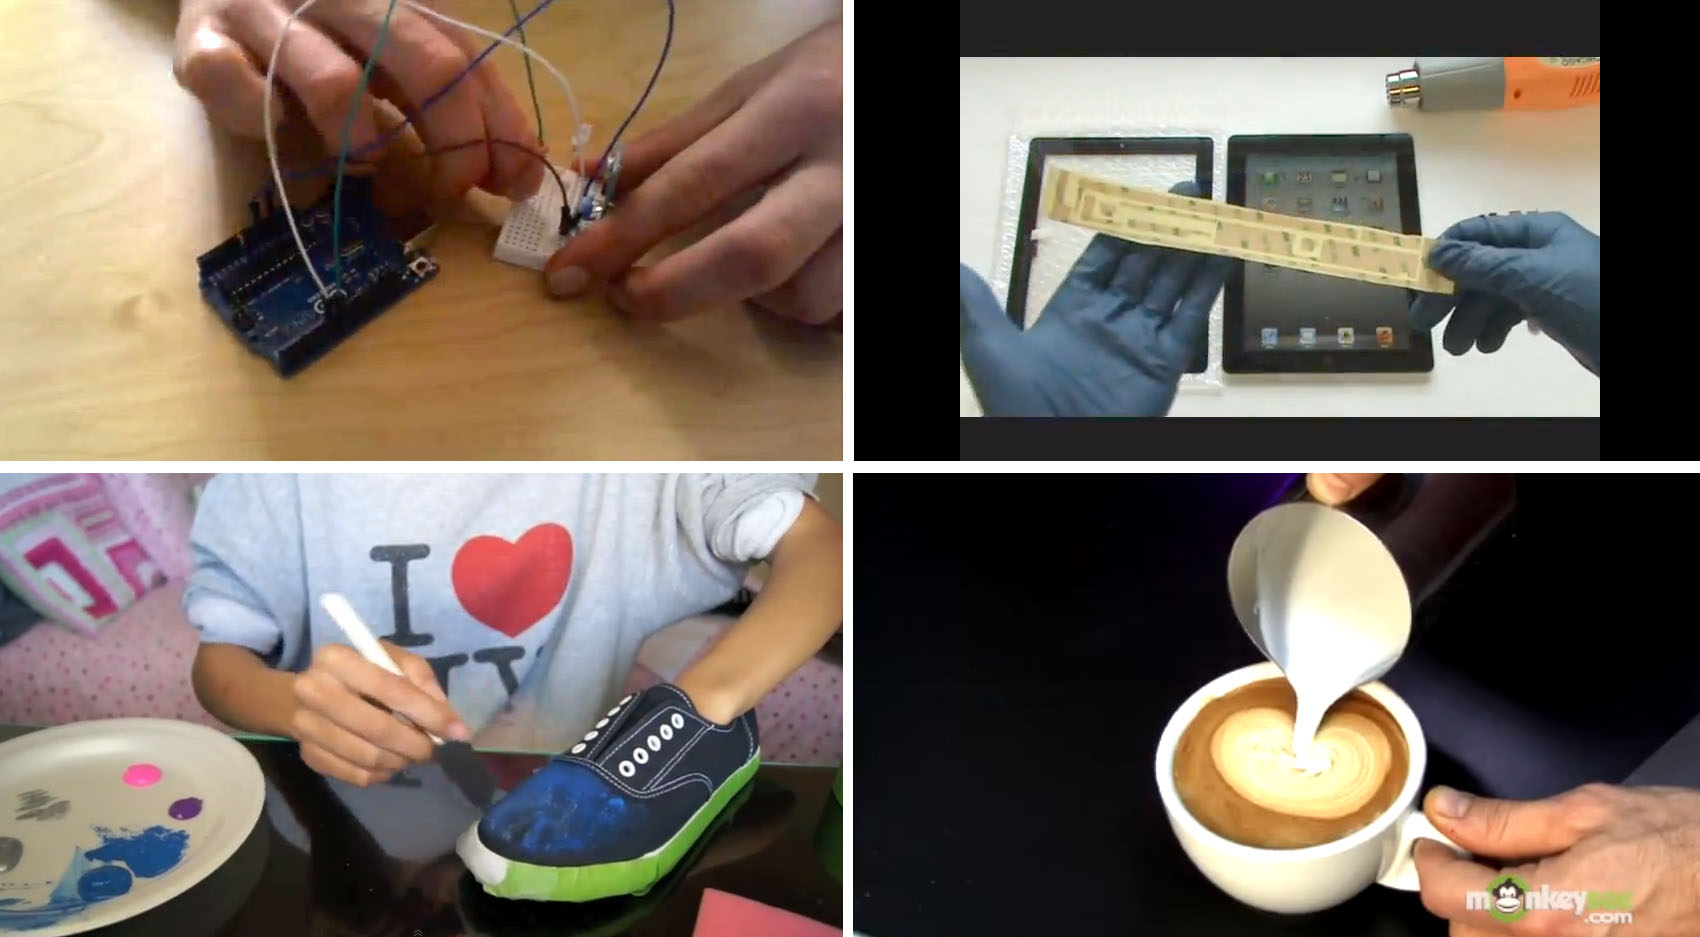
\includegraphics[width=0.7\columnwidth]{\democut/fig/formative-videostills}
  \caption{We analyzed 20 DIY instructional videos. Examples included (clockwise from top left): Microcontroller circuit design, tablet screen replacement, custom shoe painting, and creating latte art.}
  \label{fig:formative}
  \vspace{-0.25in}
\end{figure}

20 videos from 20 distinct authors were coded in a week. Figure \ref{fig:formative} presents selected examples; Appendix B preserves detailed information.
%The list of videos is available in the submitted supplemental materials.
The average length of these videos is 5 minutes and 5 seconds (\emph{max}=9'08",
\emph{min}=1'54"), and the average view count is 269,426
(\emph{max}=4,004,613, \emph{min}=1,156). Although these tutorials
cover various topics and tasks, we observed several common
characteristics of the videos:

\begin{itemize}
  \setlength{\itemsep}{0pt}

\item \subsubTitleBold{Narration} All of the videos include narration that
  explains what is happening in the tutorial. Most authors seem to
  narrate during the demonstration (70\%), while fewer authors record a
  separate voice-over track.

\item \subsubTitleBold{Speed-up effects} Most videos (60\%) include editing
  effects that speed up repetitive actions, such as screwing in
  fasteners or chopping vegetables. In many cases, authors break the
  sync between the audio and video tracks in these sped-up sections so
  that the narration plays continuously at normal speed with no long
  silences while the video plays at a faster speed.

\item \subsubTitleBold{Annotations} Many videos (65\%) include titles
  that add relevant information about the task, including descriptions
  of depicted objects or actions, measurements, elapsed time, and
  details that are not shown in the demonstration. Some videos also
  include other annotations (e.g., arrows, rectangular highlights)
  that emphasize important details.

\end{itemize}

This analysis suggests that authors apply a common set of editing
techniques. Since the final videos convey limited information
about the recording and editing processes, we
interviewed several authors of the selected videos.
We hope to learn what kind of footage they omitted and how much time they spent on editing. We also wanted to understand the rationale behind the edits.

%For example, it is not
%possible to determine what kind of footage was omitted or the amount
%of time spent editing the video. Furthermore, while the goals of some
%edits may seem obvious (e.g., annotations highlight important details
%in the video) it is difficult to infer the rationale behind all
%editing decisions. To gain more insight about the editing process, we
%interviewed several authors of the selected videos.

\subsection{Interviews with Tutorial Authors}
We contacted the 20 YouTube account holders of the analyzed videos,
and interviewed the first six who responded (all males, ages 17 to 48).
%to learn more about their recording and editing process.
One of the
YouTube user accounts corresponded to a 3-person team, which we
counted as a single participant (P6). Among the participants, two were
professional tutorial makers, while the rest were amateurs. For editing, three used Apple Final Cut Pro, two Corel VideoStudio, and one Adobe Premiere.
Table~\ref{tab:table1} summarizes other information about the
experience of the authors.
%, what categories of videos they typically create and sample projects they created.

\begin{table}
  \centering
  \small
  \begin{tabular}{|c|c|c|c|l|}
    \hline
    \tabhead{ID} &
    \multicolumn{1}{|c|}{\centering\tabhead{Category}} &
    \multicolumn{1}{|c|}{\centering\tabhead{Experience}} &
    \multicolumn{1}{|p{0.08\columnwidth}|}{\centering\tabhead{Videos}} &
    \multicolumn{1}{|c|}{\centering\tabhead{Sample Project}} \\ \hline
    P1 & electronics & professional & 48* & Body-mounted camera \\
    P2 & home/repair & amateur & 162 & Powder coating aluminum \\
    P3 & science & professional & 45* & Develop caffenol film \\
    P4 & home/repair & amateur & 717 & Snowblower repair \\
    P5 & home/repair & amateur & 33 & Paintcan setup \\
    P6 & electronics & amateur & 5 & On-beat disco light \\ \hline
  \end{tabular}
  \caption{Background information about interview participants. \emph{* Numbers of videos published on personal YouTube channels, excluding those on the professional channels.}}
  \label{tab:table1}
\end{table}

\subsubsection{Capture}
Except for the team (P6), all of the participants
record demonstrations individually without any assistants. P2--P6 use
a single video camera, while P1 uses an extra camera to capture
closeup shots. To keep the recording process simple, the amateur
authors tend to capture demonstrations in one uninterrupted take,
narrating the action as they go. Naturally, such recordings often
include mistakes (e.g., walking out of frame to retrieve a forgotten tool) and long, repetitive actions. In contrast, the
professional authors create a script beforehand and record the
narration separately.

\subsubsection{Editing}
All of the participants mentioned the importance of editing the final video tutorial down to a reasonable length (5--10 minutes). The goal is to provide enough information to understand the demonstration, but at the same time keep the video lively and interesting. P2 described his strategy as follows: \iquote{If you can get rid of it and the video content still gets through, get rid of it}; \iquote{The way to make your video sizzle is to have good cuts, good points.} As a result, authors spend much of their editing time deciding on cuts, segmenting the video, removing and merging shots, and adding visual
effects to speed up repetitive actions. They also take time to add
subtitles and annotations. As P4 explained, \iquote{the filming is the easiest part; it is the editing that's the challenge.} Overall, participants reported that filming time takes from one hour up to one day, and editing time typically takes 6--12 hours, depending on the the complexity of the project.

